\subsection{RAP-MUSIC}
Rekursiivisen lisäyksen ja projisoinnin MUSIC (recursively applied and projected MUSIC, RAP-MUSIC) \citep{Mosher1999SourceMUSIC} on MUSIC-algoritmin iteratiivinen versio, jossa löydetyn lähteen virittämä komponentti projisoidaan pois signaaliavaruudesta ennen seuraavan lähteen paikantamista. Tämän jälkeen seuraava lähde etsitään muunnetun signaaliavaruuden paikannusfunktion maksimina. RAP-MUSICin etuna on, että se löytää lähdepisteet yksi kerrallaan eikä kaikkia maksimipisteitä kerralla tavallisen MUSIC-algoritmin tapaan \citep{Makela2018TruncatedLocalization}.

%RAP-MUSIC löytää hyvin korreloituneita lähteitä tavallista MUSICia paremmin

RAP-MUSIC alkaa tavallisen MUSIC-algoritmin tapaan löytäen ensimmäisen maksimipisteen estimaatin \textbf{\^p}, jolla on topografia \textbf{l(\^p)}. Iteraatiokierrosta \textit{k}+1 varten muodostamme projektio-operaattorin, joka projisoi topografian \textbf{l(\^p)} pois signaaliavaruudesta

\begin{equation}
    \mathbf{Q}_k = \mathbf{I}-\mathbf{B}_k\mathbf{B}_k^\dagger,
\end{equation}
jossa $\mathbf{B}_k = [\mathbf{l(p}_1),...,\mathbf{l(p}_{k})]$ sisältää löydettyjen lähteiden topografiat. Tämä operaattori lisätään data-avaruuteen:

\begin{equation}
    \mathbf{Q}_k = \mathbf{Q}_k\mathbf{AS}+\mathbf{Q}_k\epsilon
\end{equation}

Muunnettu signaaliavaruus on täten $\text{span}(\mathbf{Q}_k\mathbf{U}(:,1:n))$ ja muunnetut topografiat $\mathbf{Q}_k\mathbf{l(p)}$. Tästä muunnetusta signaaliavaruudesta muodostetaan singulaariarvohajotelma

\begin{equation}
    \mathbf{Q}_k\mathbf{U}(:,1:n) = \mathbf{U}_k\mathbf{D}_k\mathbf{V}_k^T
\end{equation}

Muodostetaan projektio muunnettuun signaaliavaruuteen (\ref{eq:projektio}):
\begin{equation}
    \mathbf{P}_k = \mathbf{Q}_k\mathbf{U}(:,1:n)(\mathbf{Q}_k\mathbf{U}(:,1:n))^{\dagger} = \mathbf{U}_k(1:n)\mathbf{U}_k(1:n)^T
\end{equation}

Kiinnitetyn orientaation paikannusfunktio:
\begin{equation}
    \mathbf{\mu_k(p)} = \frac{||\mathbf{P}_k\mathbf{Q}_k\mathbf{l(p)}||^2}{||\mathbf{Q}_k\mathbf{l(p)}||^2}
    \begin{cases}
    =1\text{, jos p on lähde}\\
    <1\text{, jos p ei ole lähde}
     \end{cases}
\end{equation}

Vapaan orientaation paikannusfunktio saadaan edellisen kappaleen mukaisesti:
\begin{equation}
    \mathbf{\mu_k(p)} = \max_{||\eta||=1} \frac{||\mathbf{P}_k\mathbf{Q}_k\mathbf{L(p)\eta}||^2}{||\mathbf{Q}_k\mathbf{L(p)\eta}||^2}
    \begin{cases}
    =1\text{, jos p on lähde}\\
    <1\text{, jos p ei ole lähde}
     \end{cases}
\end{equation}


\subsubsection{RAP-dilemma}
RAP-MUSIC:n paikannusfunktio saattaa löytää lähdepisteitä jo löydettyjen lähteiden läheltä, joka johtuu siitä, ettei algoritmi pysty täysin poistamaan topografiaa löydettyjen dipolien paikalta. RAP-dilemmaa havaitaan varsinkin kohinattomalla ja valkoisen kohinan datalla. RAP-dilemman vuoksi ominaisarvoissa ei havaita selkeää pudotusta, joka voi johtaa väärään lähteiden lukumäärän arvioimiseen. \citep{Makela2018TruncatedLocalization}


\clearpage

\begin{figure}[ht]
    \centering
    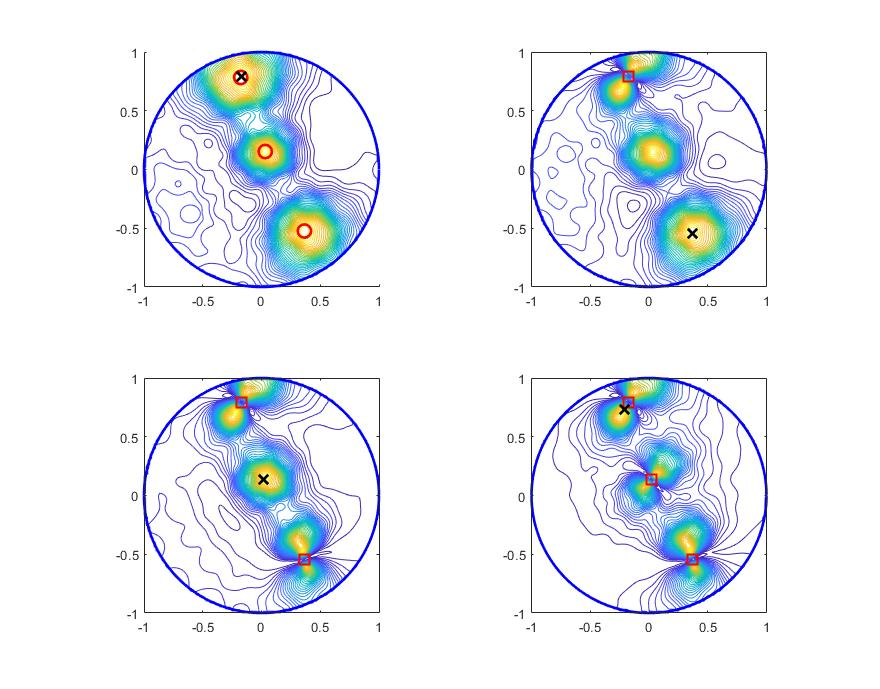
\includegraphics[width=\textwidth]{rapdilemma.jpg}
    \caption{RAP-dilemmaa havainnoillistava kuva. Kuvista huomataan suuret maksimiarvot jo löydettyjen lähteiden ympäriltä.}
    \label{fig:dilemma}
\end{figure}